\documentclass{book}
\usepackage{graphicx}
\usepackage{ctex} % Add ctex package for Chinese support
\usepackage{titlesec}
%\usepackage{titletoc} % Add titletoc package for customizing TOC
\usepackage{enumitem}

\usepackage{lipsum} % for generating dummy text, you can remove this in your final document
\usepackage{datetime}
\usepackage{circuitikz}
\usetikzlibrary{circuits}
\usetikzlibrary{circuits.plc.ladder}

\usetikzlibrary{circuits.logic.US,positioning}

% Set the document font to a font that supports both English and Chinese
\setCJKmainfont{SimSun} % Replace with an appropriate Chinese font
\setmainfont{Times New Roman} % Replace with an appropriate English font

\usepackage{titletoc}% http://ctan.org/pkg/titletoc


% Customizing TOC
\usepackage{titletoc}% http://ctan.org/pkg/titletoc
\titlecontents*{chapter}% <section-type>
[0pt]% <left>
{\addvspace{1em}}% <above-code>
{\bfseries\chaptername\ \thecontentslabel\quad}% <numbered-entry-format>
{}% <numberless-entry-format>
{\bfseries\hfill\contentspage}% <filler-page-format>


\begin{document}
	
	\frontmatter % Title page, preface, and table of contents
	
	\begin{titlepage}
		\centering
%		\vspace*{\fill}
		

	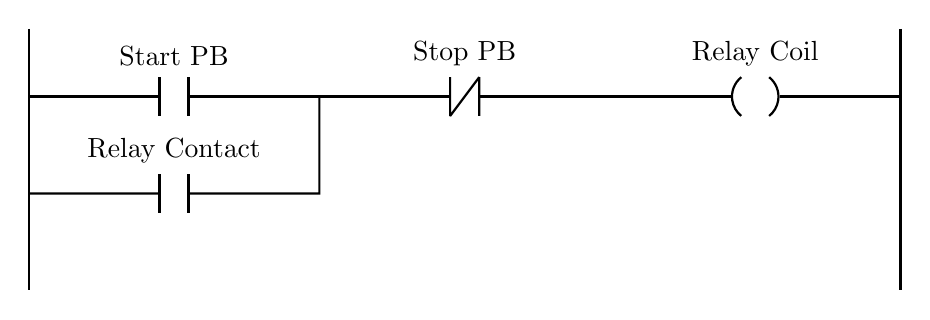
\begin{tikzpicture}[circuit plc ladder,thick,ladderrungsep=0.8]
		\draw(0,0) 
		to [contact NO={info={Start PB},name=ca}] ++(3,0)
		to [contact NC={info={Stop PB},name=ca}] ++(3,0)	
		to [coil={info={Relay Coil}}] ++(3,0) coordinate(laddertopright);
		ill[red!20] (laddertopright |- ca.south) rectangle +(-2,-1em);
		\draw(0,-1) 
		to [contact NO={info={Relay Contact},name=cb}] ++(3,0) -- +(0,1);
		ill[red!20] (laddertopright |- cb.south) 
		rectangle +(-2,-1em) coordinate (pb);
		ill[blue!20] (pb) rectangle ++(2,-0.8);
		\ladderrungend{2}
		\ladderpowerrails
		
	\end{tikzpicture}
		
	%	\includegraphics[width=0.8\textwidth]{../images/motor.png} % Replace with your image file
		\vfill
		\Huge\textbf{The Art of PLC Programming\\[10pt] PLC 程序设计的艺术}
		\vfill
%		\vspace{0.1cm}
\Large\textbf{Jeff Wang, P.Eng.}
\vfill
  \vspace{0.5cm}
\large\textit{Toronto} \monthname, \the\year% Adjust the location and date format as needed

	\end{titlepage}
	
	\chapter*{Preface 前言}
	I've long harbored the idea of penning a comprehensive book on PLC programming. The constraint of time, coupled with an insatiable appetite for continuous learning and improvement, has delayed this endeavor. With the accumulation of experiences and lessons learned, I've found inspiration in sharing both the triumphs and tribulations of programming. Thus, the genesis of this book on PLC programming was conceived.
	
	\tableofcontents
	
	\mainmatter % Main content
	
	\chapter{Overview } 

	
	PLC是Programmable Logic Controller(可编程逻辑控制) 的简写 ,PLC目前演变成为工业自动化领域的重要组成部分。最初为了简化并提升制造过程而设计,PLC如今已成为工业控制系统中不可或缺的元素。
	
	起源和演进
	
	PLC的发展可以追溯到上世纪中期,当时自动化制造概念初露端倪。工程师们致力于取代繁琐的继电器控制系统,创造了第一台PLC,标志着工业自动化领域迎来了革命性的变革。
	
	多年来,PLC不仅在硬件和编程能力方面取得了显著进展,从最初的继电器逻辑发展到如今复杂的数字控制,成为现代工业过程的关键推动力。
	广泛的工业应用
	
	如今,PLC在各个行业中都发挥着关键作用,提供卓越的效率、可靠性和多功能性。从控制工厂车间中的复杂制造过程到关键基础设施,PLC在不同领域都有着广泛的应用。
	%\lipsum[1-2] % Remove this line and add your actual content
	
	\section{什么是PLC} 
	可编程逻辑控制器(PLC)是一种专用的工业计算机,用于控制和自动化制造过程、机械设备以及各种电机机械过程。PLC设计用于在恶劣的工业环境中运行,能够承受高温、湿度和电气噪声等条件。
	
	PLC在工业自动化中至关重要,因为它们可以编程执行各种任务,如控制机械、管理生产线以及监控输入/输出信号。PLC的编程涉及创建梯形逻辑图或使用IEC 61131-3标准规定的其他编程语言。这使工程师能够根据输入条件和所需的输出行为定义控制器的行为。
	
	PLC的关键特点包括实时操作、可靠性以及与各种传感器和执行器进行接口的能力。它们已经成为现代制造过程中不可或缺的一部分,实现了提高效率、灵活性以及适应生产需求变化的能力。
	
在北美市场,PLC产品主要分为三大类,即美系(美国制造商),德系(德国制造商)和日系(日本制造商)
	
	Rockwell Automation (罗克韦尔自动化)
	产品系列:Allen-Bradley ControlLogix, CompactLogix, MicroLogix等。
	该公司提供广泛的PLC解决方案,适用于不同规模和类型的工业自动化应用。
	
	Siemens (西门子)
	产品系列:SIMATIC S7-1200, S7-1500等。
	西门子的PLC产品在制造、能源、交通等行业中应用广泛,以高性能和可靠性而闻名。
	
	Omron Corporation (欧姆龙)	
	产品系列:CP1, CJ2, NJ系列等。
	欧姆龙的PLC产品适用于各种应用,包括机械制造、医疗设备和自动化控制系统。
	
	在北美市场,PLC产品主要分为三大类,即美系(美国制造商),德系(德国制造商)和日系(日本制造商)。
	
	美系 PLC:
	以Rockwell Automation(罗克韦尔自动化)的Allen-Bradley系列为代表。
	这些PLC产品在北美市场非常流行,广泛用于各种工业自动化应用。
	
	德系 PLC:
	以Siemens(西门子)的SIMATIC系列为代表。
	德系PLC产品以其高性能、可靠性和先进的技术而著称,在工业自动化领域有着广泛的应用。
	
	日系 PLC:
	以Omron Corporation(欧姆龙)的CP1、CJ2、NJ系列为代表。
	日系PLC产品在北美市场也有一定份额,其产品在机械制造、医疗设备等领域得到广泛应用。
	
	这三大类PLC都有各自的特点和优势,企业在选择时通常会考虑到其应用需求、性能要求以及与其他设备的兼容性。
	
	此外, Beckhoff, Schneider Electric and Mitsubishi Electric出品的PLC在市场上也占有一定的份额
	%\lipsum[2-3]
	\section{PLC工作流程} 
	PLC(可编程逻辑控制器)的工作过程流程包括几个阶段,通常包括输入处理、程序执行和输出生成。以下是PLC工作过程流程的简化概述:

 	\begin{center}	
	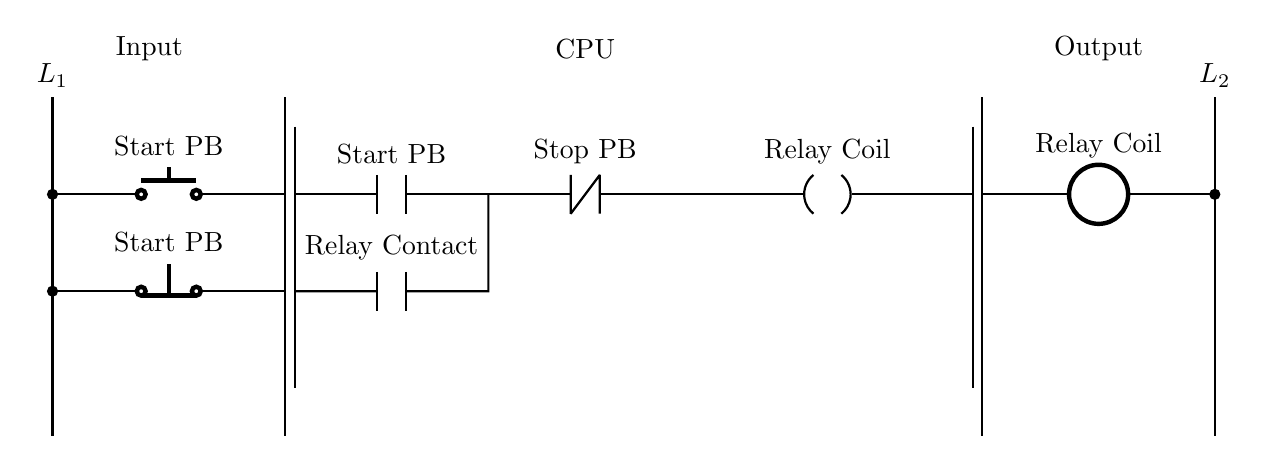
\begin{tikzpicture}[circuit plc ladder,thick,ladderrungsep=0.8]
		
		\draw (-2.5,1) node[above]{$L_1$} -- ++(0,-3.5);
		\draw (-0.1,1) node[above]{} -- ++(0,-3.5);
		\node at (-1.5,1.5){Input};		
		
		\draw (-2.5,0) node[circ]{} to [nopb=Start PB] (-0.1,0) ;
		\draw (-2.5,-1) node[circ]{} to [ncpb=Start PB] (-0.1,-1) ; 	
		
		\draw (9.5,1) node[above]{$L_2$} -- ++(0,-3.5);
		\draw (7.1,1) node[above]{} -- ++(0,-3.5);		
		\node at (8.3,1.5){Output};
		
		\draw (7.1,0) 
		%to [coil={info={Relay Coil}}] ++(2.5,0) coordinate(laddertopright) node[circ]{} ;
		to [esource,label=Relay Coil,/tikz/circuitikz/bipoles/length=1.25cm] (9.5,0) node[circ]{};
		\node at (3,1.5){CPU};	
		
		\draw(0,0) 
		to [contact NO={info={Start PB},name=ca}] ++(2,0)
		to [contact NC={info={Stop PB} ,name=ca}] ++(2,0)	
		to [coil={info={Relay Coil} }] ++(3,0) coordinate(laddertopright);
		ill[red!20] (laddertopright |- ca.south) rectangle +(-2,-1em);
		\draw(0,-1) 
		to [contact NO={info={Relay Contact},name=cb }] ++(2,0) -- +(0,1);
		ill[red!20] (laddertopright |- cb.south) 
		rectangle +(-2,-1em) coordinate (pb);
		ill[blue!20] (pb) rectangle ++(2,-0.8);
		\ladderrungend{2}
		\ladderpowerrails
		
	\end{tikzpicture}
\end{center}
\begin{figure} [ht]
	%\includegraphics[width=0.8\textwidth]{../images/motor.png} % Replace with your image file
	\caption{PLC Working Principle}
	\label{fig:plc-ladder}
\end{figure}		
	%\includegraphics[width=0.8\textwidth]{../images/motor.png} % Replace with your image file
	% need to replace with correct picture
\section*{PLC 工作过程}

\subsection*{STEP 1. 输入处理:}
\begin{itemize}
	\item \textbf{感知输入信号:} PLC 从各种传感器和设备(如开关、传感器和其他输入模块)接收输入信号。
	\item \textbf{输入信号调理:} 接收到的信号可能会经过调理,例如过滤或缩放,以确保与 PLC 内部处理的兼容性。
\end{itemize}

\subsection*{STEP 2. 程序执行:}
\begin{itemize}
	\item \textbf{程序扫描:} PLC 以循环的方式重复扫描其控制程序。每次扫描代表程序执行的一个周期。
	\item \textbf{程序执行:} 在每次扫描期间,PLC 执行存储在其内存中的用户定义的控制程序。该程序使用梯形逻辑或其他符合 IEC 61131-3 标准的编程语言编写。
	\item \textbf{数据处理:} PLC 根据程序逻辑处理输入数据,实施逻辑运算、定时器、计数器和其他控制功能。
\end{itemize}

\subsection*{STEP 3. 输出生成:}
\begin{itemize}
	\item \textbf{输出信号生成:} 根据处理后的输入数据和程序逻辑,PLC 生成输出信号。
	\item \textbf{输出信号调理:} 生成的输出信号可能会经过调理,例如放大或隔离,以适应连接的执行器和设备的要求。
	\item \textbf{输出到执行器:} 经过调理的输出信号然后发送到执行器,如电机、阀门或继电器,以控制连接的工业过程。
\end{itemize}

\subsection*{STEP 4. 重复循环:}
\begin{itemize}
	\item 整个过程以循环的方式不断重复。PLC 扫描输入,执行程序,生成输出,然后重复循环,以保持对工业过程的实时控制。
\end{itemize}

PLC 操作的这种循环和实时性质使其能够持续监控和控制制造、能源和自动化等行业的过程。PLC 的编程语言的灵活性和PLC 的适应性使其成为各种工业应用中不可或缺的部分。

	%\lipsum[4-5]
	\section{PLC常用的编程语言} 
	梯形图是业界常用的一种PLC 编程主要工具。 适合于任何水平 的从业人员进行PLC编程工作。此外,随着PLC广泛应用和适合不同场合应用PLC的发展。业界制定了一种PLC编程语言的国际标准IEC 61131-3.
	IEC 61131-3 标准是一个通用的框架,使工程师能够在不同厂家的PLC上使用相似的编程概念和语言。这样,他们可以更容易地迁移和重用代码,提高工程的灵活性和可维护性。
	该标准包括五种主要的PLC编程语言,分别是:
 
	
	\section*{IEC 61131-3 PLC 编程语言}
	
	IEC 61131-3 是一种国际标准,定义了可编程逻辑控制器(PLC)的编程语言和标准化方法。该标准包括五种主要的PLC编程语言,分别是:
	
	\begin{enumerate}[label=--]
		\item \textbf{梯形图(Ladder Diagram):}
		\begin{itemize}
			\item \textbf{描述方式:} 使用梯形图的元件,如继电器、触点、线圈,表示逻辑和控制关系。
			\item \textbf{应用领域:} 适用于传统的离散控制,易于理解和实施。
		\end{itemize}
		
		\item \textbf{结构化文本(Structured Text):}
		\begin{itemize}
			\item \textbf{描述方式:} 使用高级编程语言的结构化文本,如C或Pascal,进行逻辑编程。
			\item \textbf{应用领域:} 适用于复杂的控制算法和数学运算,提供更灵活的编程选项。
		\end{itemize}
		
		\item \textbf{功能块图(Function Block Diagram):}
		\begin{itemize}
			\item \textbf{描述方式:} 使用图形符号表示功能块,每个块执行特定的功能或运算。
			\item \textbf{应用领域:} 适用于模块化的控制系统设计,易于维护和理解。
		\end{itemize}
		
		\item \textbf{指令列表(Instruction List):}
		\begin{itemize}
			\item \textbf{描述方式:} 使用简洁的指令列表,类似于汇编语言,表示程序执行的顺序。
			\item \textbf{应用领域:} 适用于对底层硬件控制较为熟悉的工程师,可实现较高的程序执行效率。
		\end{itemize}
		
		\item \textbf{图形化编程语言(Sequential Function Chart):}
		\begin{itemize}
			\item \textbf{描述方式:} 使用图形化的图表表示程序的状态转换和顺序执行。
			\item \textbf{应用领域:} 适用于描述复杂的状态机和顺序控制,易于可视化系统行为。
		\end{itemize}
	\end{enumerate}
	
	IEC 61131-3 标准的目标是提供一个通用的框架,使工程师能够在不同厂家的PLC上使用相似的编程概念和语言。这样,他们可以更容易地迁移和重用代码,提高工程的灵活性和可维护性。
	%\lipsum[6-7]
	\chapter{简单的PLC控制程序}
 简单的PLC控制程序是为了执行基本控制任务而设计的可编程逻辑控制器(PLC)程序。这类程序通常用于自动化和监控工业过程,以实现特定的功能。PLC控制程序由PLC编程工程师编写,用于控制和监控设备、机器或生产线的运作。
	
	\textbf{主要特征:}
	\begin{enumerate}[label=--]
		\item \textbf{逻辑控制:} 简单的PLC控制程序主要包含逻辑控制部分,以根据输入条件执行相应的操作。这可能涉及开关、传感器或其他输入设备的状态监测。
		
		\item \textbf{条件判断:} 根据预定的逻辑条件,程序能够判断输入信号的状态,从而决定执行何种控制操作。条件判断可包括逻辑比较、定时器和计数器等。
		
		\item \textbf{输出生成:} 程序通过逻辑运算后生成相应的输出信号。这些输出信号用于操控执行器、电机、阀门等设备,实现控制任务的自动化。
		
		\item \textbf{简单的执行顺序:} 这类程序通常按照简单的顺序执行。PLC扫描程序的每一个周期,根据逻辑规则执行相应的控制动作。
	\end{enumerate}
	
 
	
	\newpage % Forces content to start on the next page	
	%\lipsum[10-11] % Remove this line and add your actual content
	
	\section{PLC编程涉及的基础知识} 
	在工业应用中,常见的输入输出元件包括瞬时按钮、继电器、指示灯和传感器。
	\textbf{相应的电气符号如下:}

	\begin{center}
		\begin{circuitikz} 
			\draw (2,0) to [nopb=Start PB]  ++(2,0);
			\draw (5,0) to [ncpb=Stop PB]  ++(2,0);
			\draw (8,0) to [esource,label=Relay Coil,/tikz/circuitikz/bipoles/length=1.0cm] ++(2,0) 	;
			\draw (11,0) to [lamp=Pilot Light,/tikz/circuitikz/bipoles/length=1.0cm] ++(2,0);
		\end{circuitikz}
	\end{center}
	\begin{figure} [ht]
		%\includegraphics[width=0.8\textwidth]{../images/motor.png} % Replace with your image file
		\caption{Electrical Diagram Symbols}
		\label{fig:plc-ladder}
	\end{figure}
	\textbf{相应的PLC梯形图使用的符号:}
	\begin{center}
	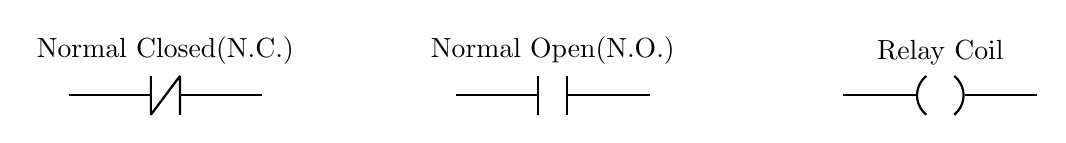
\begin{tikzpicture} [circuit plc ladder,thick,ladderrungsep=0.8]
		% Define symbols
		\draw (2,0) to [contact NC={info={Normal Closed(N.C.)},name=ca}] ++(2,0);
		\draw (6,0) to [contact NO={info={Normal Open(N.O.)} ,name=ca}] ++(2,0);			
		\draw (10,0) to [coil={info={Relay Coil}}] ++(2,0) coordinate(laddertopright);
	\end{tikzpicture}
	\end{center}
	%\centering
	\begin{figure} [ht]
		%\includegraphics[width=0.8\textwidth]{../images/motor.png} % Replace with your image file
		\caption{PLC Ladder Logic Symbols}
		\label{fig:plc-ladder}
	\end{figure}
	
	\textbf{常用的三种基本逻辑:}	
	\begin{center}	
	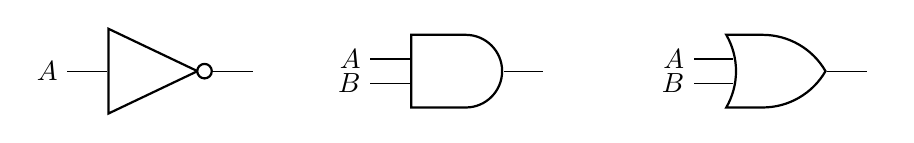
\begin{tikzpicture}[circuit logic US, every circuit symbol/.style={thick, scale=1.5}]
		% NOT gate
		\node[not gate, draw, rotate=0] (notgate) at (0,0) {};
		\draw (notgate.input) -- ++(-0.5,0) node[anchor=east] {$A$};
		\draw (notgate.output) -- ++(0.5,0) node[anchor=west] { };
		% AND gate
		\node[and gate, draw, logic gate inputs=nn] (andgate) at (4,0) {};
		\draw (andgate.input 1) -- ++(-0.5,0) node[anchor=east] {$A$};
		\draw (andgate.input 2) -- ++(-0.5,0) node[anchor=east] {$B$};
		\draw (andgate.output) -- ++(0.5,0) node[anchor=west] {};
		
		
		% OR gate
		\node[or gate, draw, logic gate inputs=nn] (orgate) at (8,0) {};
		\draw (orgate.input 1) -- ++(-0.5,0) node[anchor=east] {$A$};
		\draw (orgate.input 2) -- ++(-0.5,0) node[anchor=east] {$B$};
		\draw (orgate.output) -- ++(0.5,0) node[anchor=west] { };
		

		
	\end{tikzpicture}
\end{center}
\begin{figure} [ht]
	%\includegraphics[width=0.8\textwidth]{../images/motor.png} % Replace with your image file
	\caption{Logic Gate Symbols}
	\label{fig:Logic gate}
\end{figure}	

	\begin{center}
	\begin{tikzpicture}[circuit plc ladder,thick,ladderrungsep=0.8]
		\draw(0,0) to [contact NC={info={A},name=ca}] ++(1,0);				
		\draw(3,0) 
		to [contact NO={info={A},name=ca}] ++(1,0)
		to [contact NO={info={B},name=ca}] ++(1,0);	 
		
		\draw(7,1) to [contact NO={info={A},name=ca}] ++(1,0);
		\draw(7,0) to [contact NO={info={B},name=ca}] ++(1,0);
		\draw(7,0) to (7,1);	 
		\draw(8,0) to (8,1);	
		
		
	\end{tikzpicture}
\end{center}
\begin{figure}[!htp] 
	\centering 
	%	\includegraphics{C:/Junk/tex/nocontact.jpg}
	\caption{Ladder logic(NOT, AND, OR) }\label{fig:LD} 
\end{figure}	
	
	\newpage % Forces content to start on the next page	
	\section*{瞬时按钮开关}
	
 	瞬时按钮是一种常见的工业控制系统输入设备。与常规按钮不同,瞬时按钮在被按下的瞬间起作用,并且会自动返回原位。
 	\begin{figure} [ht]
 		   	\centering 
% 	\includegraphics[width=0.5\textwidth]{./image/pushButton.jpg} % Replace with your image file
 	%\includegraphics[width=0.8\textwidth]{../images/motor.png}
 	\caption{Momentary push buttons}
 
	 \end{figure}
%	 \begin{itemize}[label=--]
\begin{enumerate}[label=--]
 	\item \textbf{短暂触发:} 瞬时按钮仅在按下的瞬间起作用,不会保持在按下状态。
 	\item \textbf{手动操控:} 用户可以通过手动按下按钮来触发或输入信号。
 	\item \textbf{多功能用途:} 在工业环境中,瞬时按钮常用于启动、停止、复位等控制功能。
 	\item \textbf{通常闭合或通常断开:} 瞬时按钮可以设计为通常闭合(NC)或通常断开(NO),具体取决于应用的需求。
 	\item \textbf{耐用性:} 由于常常需要频繁操作,瞬时按钮通常设计为耐用和可靠的设备。
%	 \end{itemize}
  \end{enumerate}
  
   	\begin{figure} [ht]
   		   	\centering 
%  	\includegraphics[width=0.5\textwidth]{./image/NCNO.png} % Replace with your image file
  	%\includegraphics[width=0.8\textwidth]{../images/motor.png}
  	\caption{Momentary push buttons NC and NO module}
  	
  \end{figure}
  
 	\newpage % Forces content to start on the next page 
 \section*{继电器}
 
    继电器是一种电气开关,其工作原理基于电磁感应和电磁吸引。以下是对继电器工作原理的简要描述:
  	\begin{figure} [ht]
%   \begin{wrapfigure}{r}{0.4\textwidth}
   	\centering  		
%    	\includegraphics[width=0.3\textwidth]{./image/relay.jpg} % Replace with your image file
    	\caption{Relay}
% 	\end{wrapfigure}   	
   	 \end{figure}
  %\begin{enumerate}[label=\arabic*.]
\begin{enumerate}[label=--]
 	\item \textbf{电磁激励:} 继电器内部包含一个线圈(电磁线圈),当通过这个线圈通电时,产生一个磁场。
 	
 	\item \textbf{磁场引起吸引:} 产生的磁场引起继电器内的铁芯或磁性臂ature在电磁力的作用下吸引。
 	
 	\item \textbf{触点动作:} 当铁芯被吸引时,它会拉动一个机械连接,通常是一个弹簧加载的触点。这个动作改变了触点的状态,从而打开或关闭电路。
 	
 	\item \textbf{电路控制:} 继电器的触点负责控制另一电路,可以是高电流或高电压的电路。这样,继电器充当了一个低功率电路和高功率电路之间的开关。
 	
 	\item \textbf{电源去激励:} 一旦电源断开,电磁线圈中断电,磁场消失,弹簧或其他复位机制将触点返回到初始状态。
 \end{enumerate}

 	\newpage % Forces content to start on the next page  
	% example
\textbf{最简单的电气控制。 按下按钮,灯亮,松开按钮,灯灭:}	

\begin{center}	
	\begin{circuitikz}
		% Push button (NO)
		\draw (0,1) 
		to (0,3)
		to [ ] (0,2) node[circ]{};
		\draw (0,2) to [push button, l=$PB$] (4,2);
		% Pilot light
		\draw (4,2) to [lamp, l=$PL$,/tikz/circuitikz/bipoles/length=1.0cm] (8,2) node[circ]{} ;
		\draw (8,1) to (8,3); 
	\end{circuitikz}
\end{center}	

\begin{figure} [ht]
	\centering 
	\caption{Pilot light control electrical diagram}
\end{figure}

\textbf{用梯形图的程序如下:}	

	\begin{center}	
	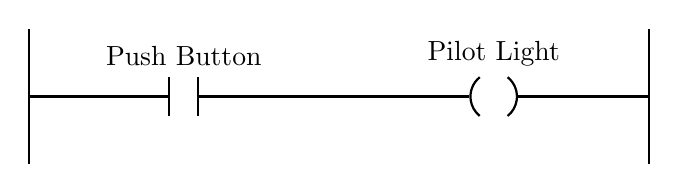
\begin{tikzpicture}[circuit plc ladder,thick,ladderrungsep=0.5]
		\draw(0,0) 
		to [contact NO={info={Push Button},name=ca}] ++(3.2,0)
		to [coil={info={Pilot Light}}] ++(3.2,0) coordinate(laddertopright);
		ill[red!20] (laddertopright |- ca.south) rectangle +(-2,-1em);
		rectangle +(-2,-1em) coordinate (pb);
		ill[blue!20] (pb) rectangle ++(2,-0.8);
		\ladderrungend{1}
		\ladderpowerrails
	\end{tikzpicture}
	\end{center}	

\begin{figure}[ht]
	\centering 
	\caption{Pilot light control ladder logic}
\end{figure}
		
\newpage % Forces content to start on the next page

	\section{电机启停PLC控制程序} 
	
工业上常用到的三相交流电机控制时,通常有两个主要电路:电源电路和控制电路。

\textbf{涉及的几个组件:}
\begin{enumerate}[label=--]
	\item \textbf{常开按钮(启动按钮):} 该按钮通常处于打开状态,按下它会启动电机的启动序列。
	
	\item \textbf{常闭按钮(停止按钮):} 该按钮通常处于关闭状态,按下它会停止电机。
	
	\item \textbf{三相继电器:} 继电器是一种电磁开关,用于控制电机的电源。它通常有三组触点,分别对应电机的三相。
	
	\item \textbf{过载保护装置:} 该装置用于保护电机免受可能损坏它的过大电流。通常是热过载继电器或磁过载继电器。
\end{enumerate}


\textbf{电源电路:}


电源电路负责向三相交流电机提供电力。它包括主接触器或起动器、过载保护装置以及电机本身等组件。
主接触器或起动器: 这个组件是一个重型继电器或接触器,能够处理电机所需的高电流。它在电源电路中充当主开关,由控制电路控制。
过载保护装置: 这些装置通常以热过载继电器或磁过载继电器的形式连接在电机电路中。它们监测电机流过的电流,通过在


		\begin{center}		
		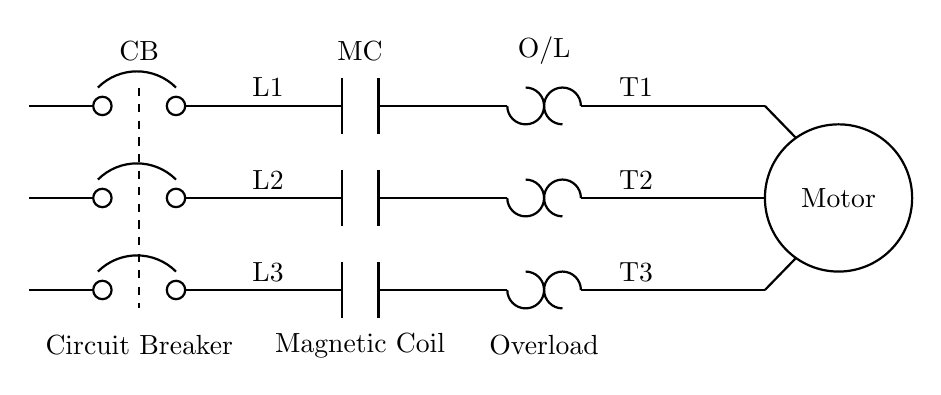
\begin{tikzpicture}[circuit plc ladder,thick,ladderrungsep=0.8,scale=0.19]
			
			% Draw a coordinate system
			%\draw[->] (-40,0) -- (40,0) node[right] {$x$};
			%\draw[->] (0,-40) -- (0,40) node[above] {$y$};	
			%\draw (-9,0) to [contact NO] (-6,0) ;
			
			%draw N.O. relay		
			%draw N.O. relay	
			%draw N.O. relay	
			
			% Set the coordinates for the line
			\coordinate (start) at (-9,1.5);
			\coordinate (end) at (-9,-1.5);
			% Draw the red V-line
			\draw (start) -- (end);
			% Set the coordinates for the line
			\coordinate (start) at (-11,1.5);
			\coordinate (end) at (-11,-1.5);
			% Draw the red V-line
			\draw (start) -- (end);		
			
			% Set the coordinates for the line
			\coordinate (start) at (-9,0);
			\coordinate (end) at (-4,0);
			% Draw the red V-line
			\draw (start) -- (end);
			% Set the coordinates for the line
			\coordinate (start) at (-11,0);
			\coordinate (end) at (-16,0);
			% Draw the red V-line
			\draw  (start) -- (end);
			
			
			
			% Set the coordinates for the line
			\coordinate (start) at (-9,6.5);
			\coordinate (end) at (-9,3.5);
			% Draw the red V-line
			\draw (start) -- (end);
			% Set the coordinates for the line
			\coordinate (start) at (-11,6.5);
			\coordinate (end) at (-11,3.5);
			% Draw the red V-line
			\draw (start) -- (end);
			
			% Set the coordinates for the line
			\coordinate (start) at (-9,5);
			\coordinate (end) at (-4,5);
			% Draw the red V-line
			\draw (start) -- (end);
			% Set the coordinates for the line
			\coordinate (start) at (-11,5);
			\coordinate (end) at (-16,5);
			% Draw the red V-line
			\draw (start) -- (end);
			
			% Set the coordinates for the line
			\coordinate (start) at (-9,-6.5);
			\coordinate (end) at (-9,-3.5);
			% Draw the red V-line
			\draw (start) -- (end);
			% Set the coordinates for the line
			\coordinate (start) at (-11,-6.5);
			\coordinate (end) at (-11,-3.5);
			% Draw the red V-line
			\draw (start) -- (end);
			
			% Set the coordinates for the line
			\coordinate (start) at (-9,-5);
			\coordinate (end) at (-4,-5);
			% Draw the red V-line
			\draw (start) -- (end);
			% Set the coordinates for the line
			\coordinate (start) at (-11,-5);
			\coordinate (end) at (-16,-5);
			% Draw the red V-line
			\draw (start) -- (end);	
			
			% draw OL
			% draw OL		
			% draw OL
			
			% Set the center and radius of the arc
			\coordinate (center) at (-2,1);
			\def\radius{1}
			
			% Draw the arc
			\draw (center) ++(0:\radius) arc (90:-180:\radius);
			
			% Optional: Mark the center
			%	\filldraw (center) circle (2pt) node[below right, black] {$(x_0, y_0)$};
			
			% Set the coordinates for the line
			\coordinate (start) at (-4,0);
			\coordinate (end) at (-2,0);
			
			% Draw the red line
			\draw (start) -- (end);
			
			%draw second OL on top
			
			% Set the center and radius of the arc
			\coordinate (center) at (-2,6);
			\def\radius{1}
			
			% Draw the arc
			\draw (center) ++(0:\radius) arc (90:-180:\radius);
			
			% Optional: Mark the center
			%	\filldraw (center) circle (2pt) node[below right, black] {$(x_0, y_0)$};
			
			% Set the coordinates for the line
			\coordinate (start) at (-4,5);
			\coordinate (end) at (-2,5);
			
			% Draw the red line
			\draw (start) -- (end);	
			
			%draw third OL on bottom
			
			% Set the center and radius of the arc
			\coordinate (center) at (-2,-4);
			\def\radius{1}
			
			% Draw the arc
			\draw (center) ++(0:\radius) arc (90:-180:\radius);
			
			% Optional: Mark the center
			%	\filldraw (center) circle (2pt) node[below right, black] {$(x_0, y_0)$};
			
			% Set the coordinates for the line
			\coordinate (start) at (-4,-5);
			\coordinate (end) at (-2,-5);
			
			% Draw the red line
			\draw (start) -- (end);	
			
			
			% Draw right OL		
			\coordinate (center) at (0,-1);
			\def\radius{1}
			
			% Draw the arc
			\draw (center) ++(0:\radius) arc (270:0:\radius);
			% Optional: Mark the center
			%	\filldraw (center) circle (2pt) node[below right, black] {$(x_1, y_1)$};		
			% Set the coordinates for the line
			\coordinate (start) at (2,0);
			\coordinate (end) at (6,0);
			
			% Draw the red line
			\draw (start) -- (end);	
			
			% Draw top the arc
			
			\coordinate (center) at (0,4);
			\def\radius{1}		
			
			\draw (center) ++(0:\radius) arc (270:0:\radius);
			% Optional: Mark the center
			%\filldraw (center) circle (2pt) node[below right, black] {$(x_1, y_1)$};		
			% Set the coordinates for the line
			\coordinate (start) at (2,5);
			\coordinate (end) at (6,5);
			
			% Draw the red line
			\draw (start) -- (end);			
			
			% Draw bottom the arc
			
			\coordinate (center) at (0,-6);
			\def\radius{1}		
			
			\draw (center) ++(0:\radius) arc (270:0:\radius);
			% Optional: Mark the center
			%\filldraw (center) circle (2pt) node[below right, black] {$(x_1, y_1)$};		
			% Set the coordinates for the line
			\coordinate (start) at (2,-5);
			\coordinate (end) at (6,-5);
			
			% Draw the red line
			\draw (start) -- (end);	
			
			%draw three phase motor
			%draw three phase motor
			%draw three phase motor
			
			
			% Set the coordinates for the line
			\coordinate (start) at (6,-5);
			\coordinate (end) at (12,-5);
			
			% Draw the blue line
			
			\draw(start) -- (end);	
			
			\draw(end) -- (13.7,-3.25);
			
			% Set the coordinates for the line
			\coordinate (start) at (6,0);
			\coordinate (end) at (12,0);
			
			% Draw the red line
			\draw(start) -- (end);
			
			% Set the coordinates for the line
			\coordinate (start) at (6,5);
			\coordinate (end) at (12,5);
			
			% Draw the red line
			\draw(start) -- (end);
			
			\draw(end) -- (13.7,3.25);
			
			%draw a circle
			%draw a circle
			%draw a circle
			
			\draw(16,0) circle [radius=4] node at (16,0) {Motor};
			% add OL and MC
			
			\node at (0,8) {O/L};
			\node at (0,-8) {Overload};
			
			\node at (-10,8) {MC}; 
			\node at (-10,-8) {Magnetic Coil}; 	 
			
			% add L1/L2/L3		
			\node at (-15,6) {L1};  
			\node at (-15,1) {L2}; 
			\node at (-15,-4) {L3};  
			
			% add T1/T2/T3		
			\node at (5,6) {T1};  
			\node at (5,1) {T2}; 
			\node at (5,-4) {T3};  
			
			
			
			% draw circuit breaker 
			
			\draw(-20,0) circle [radius=0.5] ;
			\draw(-24,0) circle [radius=0.5] ; 
			% Set the center and radius of the arc
			\coordinate (center) at (-23,1);
			\def\radius{3}
			
			% Draw the arc
			\draw (center) ++(0:\radius) arc (45:135:\radius); 
			%-----------------------------------------------
			\draw(-20,5) circle [radius=0.5] ;
			\draw(-24,5) circle [radius=0.5] ; 
			% Set the center and radius of the arc
			\coordinate (center) at (-23,6);
			\def\radius{3}
			
			% Draw the arc
			\draw (center) ++(0:\radius) arc (45:135:\radius);  
			%-----------------------------------------------
			\draw(-20,-5) circle [radius=0.5] ;
			\draw(-24,-5) circle [radius=0.5] ; 
			% Set the center and radius of the arc
			\coordinate (center) at (-23,-4);
			\def\radius{3}
			
			% Draw the arc
			\draw (center) ++(0:\radius) arc (45:135:\radius); 
			%-----------------------------------------------
			
			
			% Set the coordinates for the line
			\coordinate (start) at (-19.5,0);
			\coordinate (end) at (-16,0);
			% Draw the red V-line
			\draw (start) -- (end);
			
			% Set the coordinates for the line
			\coordinate (start) at (-24.5,0);
			\coordinate (end) at (-28,0);
			% Draw the red V-line
			\draw (start) -- (end);
			%-----------------------------------------------
			
			% Set the coordinates for the line
			\coordinate (start) at (-19.5,5);
			\coordinate (end) at (-16,5);
			% Draw the red V-line
			\draw (start) -- (end);
			
			% Set the coordinates for the line
			\coordinate (start) at (-24.5,5);
			\coordinate (end) at (-28,5);
			% Draw the red V-line
			\draw (start) -- (end);
			%-----------------------------------------------
			
			% Set the coordinates for the line
			\coordinate (start) at (-19.5,-5);
			\coordinate (end) at (-16,-5);
			% Draw the red V-line
			\draw (start) -- (end);
			
			% Set the coordinates for the line
			\coordinate (start) at (-24.5,-5);
			\coordinate (end) at (-28,-5);
			% Draw the red V-line
			\draw (start) -- (end);
			%-----------------------------------------------  
			% Set the coordinates for the line
			\coordinate (start) at (-22,6);
			\coordinate (end) at (-22,-6);		
			\draw[dashed, black] (start) -- (end) node at (-22,-8) {Circuit Breaker};		
			%\node at (-10,-8) {Magnetic Coil}; 	
			\node at (-22,8) {CB}; 
			%\node at (-10,-8) {Magnetic Coil}; 			
		\end{tikzpicture}
	\end{center}	
	
	
	\begin{figure} [ht]
		
		\caption{The power circuit Diagram}
		
	\end{figure}
	\newpage % Forces content to start on the next page
	
 
控制电路:

控制电路负责启动和停止电机,这个控制电路既可以用传统的常开按钮和常闭按钮实现,也可以用PLC完成。

传统的电机控制电路如下:
\begin{center}

\begin{circuitikz} 
	
	\draw (0,1) to (0,5)
	
	to [ ] (0,4) node[circ]{}
	to [ncpb=Stop PB] (2,4)
	
	to [nopb=Start PB] (4,4)
	
	to [esource,label=Coil,/tikz/circuitikz/bipoles/length=1.25cm] (7,4) 
	to [C= O/L,/tikz/circuitikz/bipoles/length=1.25cm,style={color=black}] (9,4) node[circ]{};
	\draw (8.3,4.4) --(7.6,3.6);
	
	\draw (2,4) node[circ]{} --(2,2)  
	to [C= MC,/tikz/circuitikz/bipoles/length=1.25cm,style={color=black}] (4,2);
	\draw (4,2)--(4,4) node[circ]{} ;
	\draw (9,1) to (9,5);
	
	
	\node at (5.5,4) {MC};
	\node at (3.0,1.2) {N.O. Contact};
	\node at (0,5.5) {$L_1$};
	\node at (9,5.5) {$L_2$};		
\end{circuitikz}

\end{center}
	\begin{figure} [ht]
	
	\caption{The control circuit Diagram}
	
\end{figure}
\textbf{传统的电机控制电路工作原理如下:}
\begin{enumerate}
	\item \textbf{电机启动序列:}
	\begin{itemize}
		\item 按下常开的启动按钮会完成电路,向三相继电器的线圈提供电源。
		\item 继电器线圈激活,其触点闭合,使电流流向电机绕组,启动电机。
	\end{itemize}
	
	\item \textbf{电机运行:}
	\begin{itemize}
		\item 一旦电机启动,常开的启动按钮可以释放。只要常闭的停止按钮没有被按下,继电器就会保持激活状态。
	\end{itemize}
	
	\item \textbf{电机停止序列:}
	\begin{itemize}
		\item 按下常闭的停止按钮会打断电路,切断电源供应到继电器线圈。
		\item 继电器失去激活状态,其触点打开,切断电源供应到电机,将其停止。
	\end{itemize}
	
	\item \textbf{过载保护:}
	\begin{itemize}
		\item 过载保护装置不断监测电机流过的电流。如果电流超过预设阈值,表示可能存在过载,过载继电器会打开其触点。
		\item 打开触点会打断电路,使继电器线圈失去激活状态,停止电机以防止损坏。
	\end{itemize}
\end{enumerate}

	这种控制电路确保对三相交流电机进行安全和受控的启动/停止序列,同时提供过载保护,以防止电机受到过大电流的损害。	在设计和实施此类电路时,请始终遵循安全准则和电气规范。

	\newpage % Forces content to start on the next page

\textbf{使用PLC的控制电路如下:}

使用PLC来控制三相交流电动机的启停在灵活性、编程简易性、减少布线复杂性、先进监测能力以及适应不断发展的系统需求等方面提供了一系列的优势。这些优势有助于提高工业应用中电机驱动系统的效率、可靠性和维护性。
		\begin{center}
		
		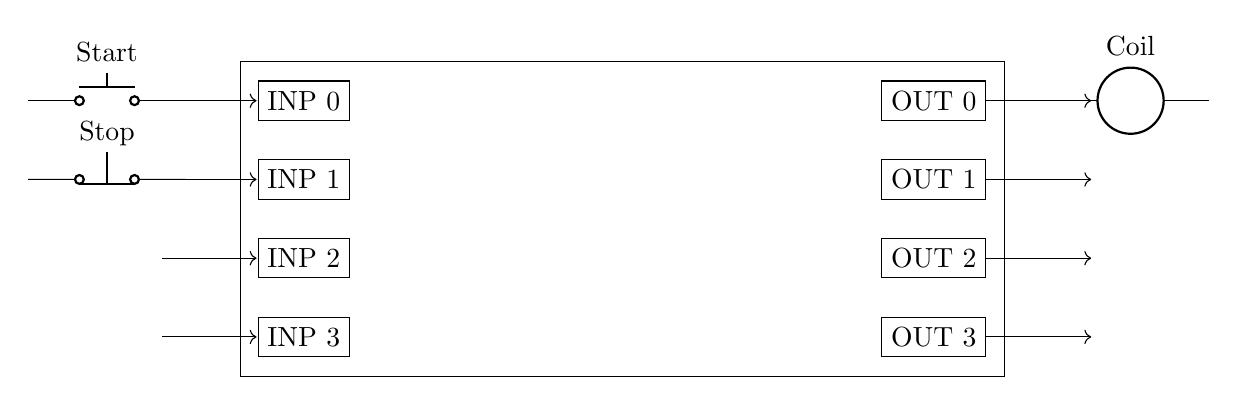
\begin{tikzpicture}
			\draw (-0.8,4) rectangle (8.9,8);
			% Define the box style
			\tikzstyle{mybox} = [draw, rectangle, minimum width=0.5cm, minimum height=0.5cm];
			
			% Draw 4 identical boxes at assigned locations
			\foreach \i/\x/\y in {0/0/7.5, 1/0/6.5 , 2/0/5.5, 3/0/4.5}
			\draw [->] (-1.8,\y) -- (-0.6,\y) node[mybox] at (\x, \y) {INP \i};
			
			\draw (-3.5,7.5) to [nopb, l=Start, n=nopb] ++(2,0);
			\draw (-3.5,6.5) to [ncpb, l=Stop, n=ncpb] ++(2,0);
			%\draw (-3.5,5.5) to [nopb, l=Start, n=nopb] ++(2,0);
			%\draw (-3.5,4.5) to [ncpb, l=Stop, n=ncpb] ++(2,0);	
			
			% Draw 4 identical boxes at assigned locations
			\foreach \i/\x/\y in {0/8/7.5, 1/8/6.5 , 2/8/5.5, 3/8/4.5}
			\draw [->] (8.65,\y) -- (10,\y) node[mybox] at (\x, \y) {OUT \i};
			
			\draw (9.5,7.5) to [esource, l=Coil] ++(2,0);
			%	\draw (9.5,5.5) to [lamp, l=PL] ++(2,0);
		\end{tikzpicture}
		
	\end{center}
	\begin{figure}[ht]
		\centering
		%\includegraphics[width=2cm]{example-image-a}
		\caption{Typical PLC motor control diagram}
	\end{figure}	
	
使用可编程逻辑控制器(PLC)来控制三相交流电动机的启停具有多项优势。以下是其中一些主要优势:

\begin{enumerate}[label=\--]
	\item \textbf{控制灵活性:} \\
	PLC提供了高度的编程灵活性,允许进行复杂的控制序列、逻辑操作和条件动作。在处理复杂的电机控制场景时,这种灵活性尤为有利。
	
	\item \textbf{编程简便性:} \\
	PLC使用梯形图或其他图形化编程语言,这些语言直观且易于理解。与传统的硬连线继电器逻辑相比,这使得编程和修改电机控制序列变得更加简便。
	
	\item \textbf{减少布线复杂性:} \\
	PLC通过用一个可编程设备替代大量离散的继电器、计时器和其他控制元件,有助于减少布线复杂性。这不仅简化了控制面板,还使故障排除和维护更加简单。
	
	\item \textbf{监测和诊断:} \\
	PLC通常具有内置的监控和诊断功能。电机参数,如电流、电压和温度,可以轻松监测。可以编程设置警报和警告,及时通知操作人员可能出现的问题,促使及时维护。
	
	\item \textbf{远程监控与控制:} \\
	配备通信功能的PLC实现了对电机的远程监控和控制。这对于分布在广大区域或难以访问的位置的系统尤为有利。
	
	\item \textbf{序列和联锁:} \\
	PLC擅长执行序列和联锁操作。这对于确保在允许电机启动或停止之前满足某些条件至关重要,以防止不安全或不可取的情况发生。
	
	\item \textbf{软启动和停机:} \\
	PLC可以实施软启动和停机序列,逐渐提高或降低电机速度。这减少了对电机及相关设备的机械和电气应力,延长了它们的寿命。
	
	\item \textbf{能效:} \\
	PLC可以实施节能的控制策略。例如,它们可以根据负载条件优化电机运行,确保电机以所需速度运行而不消耗不必要的能量。
	
	\item \textbf{与其他系统的集成:} \\
	PLC可以轻松与其他自动化和控制系统集成,如SCADA(监控与数据采集)系统。这种集成提高了工业过程整体的效率和协调性。
	
	\item \textbf{适应性:} \\
	随着工业过程的演变,PLC提供了在不进行重大硬件修改的情况下适应变化需求的灵活性。这种适应性对于面临不断变化的运营需求的行业至关重要。
\end{enumerate}

\newpage % Forces content to start on the next page

	
	\section {理解PLC程序中使用的one-shot}
 
One-Shots(单脉冲)是PLC程序中非常重要的一部分,这是因为处理器在扫描其程序时达到的惊人速度。,I/O 的扫描时间一般为纳秒(us)级别。应用程序扫描一般为微秒级别(ms). 下面是工业应用项目的扫描时间案例
	
		\begin{figure}[ht]
		\centering
		\includegraphics[scale=.85]{./image/AB_Scan2.png}
		\caption{Rockwell Automation/Allen-Bradley CompactLogix 5380 Controller}
		\end{figure}
		
	典型的一个按键动作大约持续500ms左右。用10Hz(100ms)的脉冲测试,简单一个按键动作会得到4-5个脉冲波计数。
同样条件测试,加入 one-shot 控制。 每次按键,输出都是一个单脉冲。	
工业上常用到的 toggle Switch 和 FIFO 操作经常需要这个功能	
\newpage % Forces content to start on the next page		
下面是一个Toggle Switch的PLC实例:
OFF position
	\begin{figure}[ht]
		\centering
		\includegraphics[scale=.70]{./image/toggle_OFF.png}
		\caption{Tia Portal: Toggle Switch OFF}
	\end{figure}
\newpage % Forces content to start on the next page	
ON position
	\begin{figure}[ht]
	\centering
	\includegraphics[scale=.70]{./image/toggle_ON.png}
	\caption{Tia Portal: Toggle Switch ON}
	\end{figure}
	
\newpage % Forces content to start on the next page	
	\section{矩形脉冲波生成程序} %\lipsum[13-14]	
	使用定时器来去抖动(push button debounce)按钮是PLC编程中的常见实践,以过滤在按下按钮时可能发生的噪声或抖动效应。 
	将开关或按钮连接到数字电路时,通常(几乎总是)会出现一些讨厌的问题
	
	接触弹跳现象。
	
	问题显而易见。没有一个简单、干净的低到高的过渡。如果微控制器足够快,它会将此开关事件视为多次按下按钮。
	
	
	Program PLC Input Debounce On and Off
	
	\chapter{PLC编程概念} %\lipsum[20-21] % Remove this line and add your actual content
	
	\section{输入输出} \lipsum[22-23]
	\section{简单的运算逻辑} \lipsum[24-25]
	\section{常用算法和示例-FIFO,Complexer} \lipsum[26-27]	
	
    \chapter{UI设计规范	} \lipsum[30-31] % Remove this line and add your actual content	

	\section{按钮:用HMI按钮控制电机} \lipsum[32-33]
	\section{输入数据:} \lipsum[34-35]
	\section{HMI, PI, TV} \lipsum[36-37]		

	
	\chapter{与PLC连接的设备	} \lipsum[40-41] % Remove this line and add your actual content	
	\section{常用的AS设备} \lipsum[42-43]	
	\section{条码扫描设备-Cognex} \lipsum[42-43]
	\section{控制机器人-Fanuc} \lipsum[44-45]
	\section{机器视觉识别-Cognex} \lipsum[46-47]	
	\section{运动控制-VFD和伺服} \lipsum[48-49]		
	
	\chapter{综合案例分析	} \lipsum[50-51] % Remove this line and add your actual content	

	\section{PLC框架} \lipsum[52-53]
	\section{SCADA/Ignition} \lipsum[54-55]
	% Appedix
	\chapter{附录	} \lipsum[60-61] % Remove this line and add your actual content	
	\section{索引} \lipsum[62-63]
	\section{参考文献} \lipsum[64-65] 		
		
	% Add more chapters as needed	
\end{document}
